% LaTeX source for textbook ``How to think like a computer scientist''
% Copyright (C) 1999  Allen B. Downey

% This LaTeX source is free software; you can redistribute it and/or
% modify it under the terms of the GNU General Public License as
% published by the Free Software Foundation (version 2).

% This LaTeX source is distributed in the hope that it will be useful,
% but WITHOUT ANY WARRANTY; without even the implied warranty of
% MERCHANTABILITY or FITNESS FOR A PARTICULAR PURPOSE.  See the GNU
% General Public License for more derestos.

% Compiling this LaTeX source has the effect of generating
% a device-independent representation of a textbook, which
% can be converted to other formats and printed.  All intermediate
% representations (including DVI and Postscript), and all printed
% copies of the textbook are also covered by the GNU General
% Public License.

% This distribution includes a file named COPYING that contains the text
% of the GNU General Public License.  If it is missing, you can obtain
% it from www.gnu.org or by writing to the Free Software Foundation,
% Inc., 59 Temple Place - Suite 330, Boston, MA 02111-1307, USA.


\chapter{Listas enlazadas}
\label{lista}
\index{lista}

\section{Referencias incrustadas}
\index{referencia}
\index{referencia incrustada}
\index{referencia!incrustada}
\index{lista enlazada}
\index{lista!enlazada}
\index{nodo}
\index{carga}

Hemos visto ejemplos de atributos (denominados  {\bf referencias incrustadas}) que se refieren a otros objetos  en la sección \ref{embedded}. Una estructura
de datos muy común (la {\bf lista enlazada}), toma ventaja de esta posibilidad.

Las listas enlazadas están hechas de {\bf nodos}, que contienen una referencia
al siguiente nodo en la lista. Además, cada nodo contiene una información
denominada la {\bf carga}.

Una lista enlazada se considera como  una {\bf estructura de datos recursiva} si 
damos la siguiente definición.

\begin{quote}
Una lista enlazada es:
\begin{itemize}

\item la lista vacía, representada por el valor \texttt{None}, o

\item un nodo que contiene una carga y una referencia a una lista enlazada.

\end{itemize}

\end{quote}

\index{estructura de datos recursiva}
\index{estructura de datos!recursiva}

Las estructuras de datos recursivas se implementan naturalmente con métodos
recursivos.


\section{La clase \texttt{Nodo} }
\index{clase Nodo}
\index{clase!Nodo}

Empezaremos con los métodos básicos de inicialización y 
el  \texttt{\_\_str\_\_} para que podamos crear y desplegar 
objetos:

\beforeverb
\begin{verbatim}
class Nodo:
  def __init__(self, carga=None, siguiente=None):
    self.carga = carga
    self.siguiente  = siguiente

  def __str__(self):
    return str(self.carga)
\end{verbatim}
\afterverb
%
Los parámetros para el método de inicialización son opcionales. Por defecto
la carga y el enlace \texttt{siguiente}, reciben el valor \texttt{None}.

La representación textual de un nodo es la representación de la carga.
Como cualquier valor puede ser pasado a la función \texttt{str}
, podemos almacenar cualquier tipo de valor en la lista.

Para probar la implementación, podemos crear un  \texttt{Nodo}
e imprimirlo:

\beforeverb
\begin{verbatim}
>>> nodo = Nodo("test")
>>> print nodo
test
\end{verbatim}
\afterverb
%
Para hacerlo más interesante, vamos a pensar en una lista
con varios nodos:

\beforeverb
\begin{verbatim}
>>> nodo1 = Nodo(1)
>>> nodo2 = Nodo(2)
>>> nodo3 = Nodo(3)
\end{verbatim}
\afterverb
%
Este código crea tres nodos, pero todavía no tenemos una lista 
porque estos no estan {\bf enlazados}.  El diagrama de estados
luce así:

\beforefig
\centerline{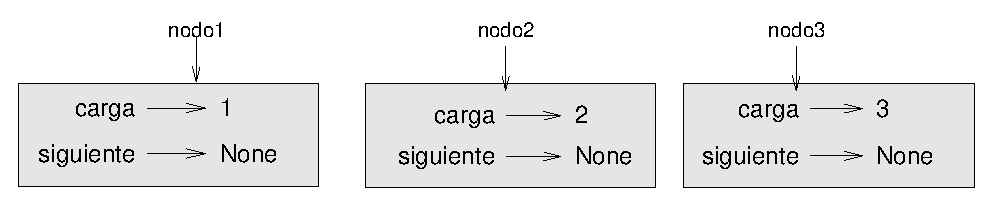
\includegraphics[scale=0.7]{illustrations/link1.eps}}
\afterfig

Para enlazar los nodos, tenemos que lograr que el primer nodo
se refiera al segundo, y que el segundo se refiera al tercero:

\beforeverb
\begin{verbatim}
>>> nodo1.siguiente = nodo2
>>> nodo2.siguiente = nodo3
\end{verbatim}
\afterverb
%
La referencia del tercer nodo es \texttt{None}, lo que indica que
es el último nodo de la lista. Ahora el diagrama de estados luce
así:

\beforefig
\centerline{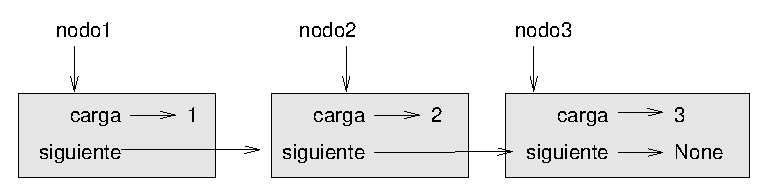
\includegraphics[scale=0.9]{illustrations/link2.eps}}
\afterfig

Ahora usted sabe cómo crear nodos y enlazarlos para crear listas.
Lo que todavía no está claro, es el por qué hacerlo.


\section{Listas como colecciones}
\index{colección}

Las listas son útiles porque proporcionan una forma de ensamblar
múltiples objetos en una entidad única, a veces llamada {\bf colección}.  En el
ejemplo, el primer nodo de la lista sirve como referencia a toda la lista.

\index{lista!imprimir}
\index{lista!como parámetro}

Para pasar la lista como parámetro, sólo tenemos que pasar una referencia
al primer nodo. Por ejemplo, la función  \texttt{imprimirLista} toma un
solo nodo como argumento. Empieza con la cabeza de la lista, imprime cada
nodo hasta llegar al final:

\beforeverb
\begin{verbatim}
def imprimirLista(nodo):
  while nodo:
    print nodo,
    nodo = nodo.siguiente
  print
\end{verbatim}
\afterverb
%
Para llamar este método, pasamos una referencia al primer nodo:

\beforeverb
\begin{verbatim}
>>> imprimirLista(nodo1)
1 2 3
\end{verbatim}
\afterverb
%
Dentro de \texttt{imprimirLista} tenemos una referencia al primer nodo 
de la lista, pero no hay variable que se refiera a los otros nodos. Tenemos
que usar el valor \texttt{siguiente} de cada nodo para obtener el siguiente
nodo.

Para recorrer una lista enlazada, es muy común usar una variable de ciclo
como \texttt{nodo} para que se refiera a cada uno de los nodos en cada 
momento.

\index{variable de ciclo}
\index{lista!recorrido}
\index{recorrido}

Este diagrama muestra el valor de \texttt{lista} y los valores que \texttt{nodo}
 toma:

\beforefig
\centerline{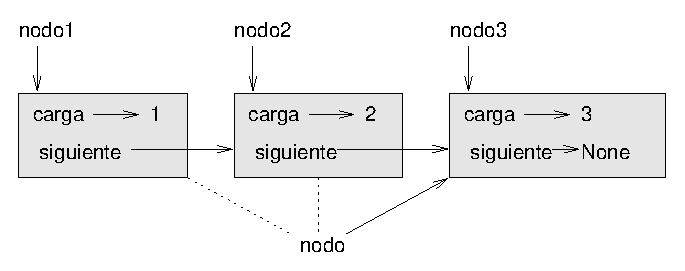
\includegraphics{illustrations/link3.eps}}
\afterfig

\begin{quote}
{\em Por convención, las listas se imprimen entre corchetes y los elementos
se separan por medio de comas, como en el ejemplo \texttt{[1, 2, 3]}.  Como 
ejercicio modifique \texttt{imprimirLista} de forma que muestre la salida
en este formato.}
\end{quote}


\section{Listas y recursión}
\label{listrecursion}
\index{lista!recorrido recursivo}
\index{recorrido}

Es natural implementar muchas operaciones sobre listas por medio de 
métodos recursivos. Por ejemplo, el siguiente algoritmo recursivo
imprime una lista al revés:

\begin{enumerate}

\item Separe la lista en dos partes: el primer nodo (la cabeza de la
lista); y el resto.

\item Imprima el resto al revés.

\item Imprima la cabeza.

\end{enumerate}

Por supuesto, el paso 2, el llamado recursivo asume que ya tenemos una
forma de imprimir una lista al revés. Si asumimos que esto es así 
---el salto de fe---entonces podemos convencernos de que el algoritmo
trabaja correctamente.

\index{salto de fe}
\index{listas!imprimiendo al revés}

Todo lo que necesitamos es un caso base y una forma de demostrar que
para cualquier lista, eventualmente llegaremos al caso base. Dada la
definición recursiva de una lista, un caso base natural es la lista 
vacía, representada por \texttt{None}:

\beforeverb
\begin{verbatim}
def imprimirAlReves(lista):
  if lista == None: 
    return
  cabeza = lista
  resto = lista.siguiente
  imprimirAlReves(resto)
  print cabeza,
\end{verbatim}
\afterverb
%
La primera línea resuelve el caso base. Las siguientes separan
la  \texttt{cabeza} y el \texttt{resto}. Las últimas dos líneas
imprimen la lista. La coma al final de la última línea evita que
Python introduzca una nueva línea después de cada nodo.

Ahora llamamos a este método:

\beforeverb
\begin{verbatim}
>>> imprimirAlReves(nodo1)
3 2 1
\end{verbatim}
\afterverb
%
El efecto es una impresión la lista, al revés.

Una pregunta natural que usted se puede estar formulando es, ¿por qué razón
\texttt{imprimirAlReves} e \texttt{imprimirLista} son funciones y no 
métodos en la clase \texttt{Nodo}? La razón es que queremos usar a
 \texttt{None} para representar la lista vacía y no se puede llamar
un método sobre  \texttt{None} en Python. Esta limitación hace un 
poco engorroso escribir el código para manipulación de listas 
siguiendo la programación orientada a objetos.

¿Podemos demostrar que  \texttt{imprimirAlReves} va a terminar siempre? 
En otras palabras, ¿llegará siempre al caso base? De hecho, la respuesta
es negativa, algunas listas causarán un error de ejecución.


\section{Listas infinitas }
\index{lista infinita}
\index{lista!infinita}
\index{ciclos!en listas}
\index{lista!ciclo}

No hay manera de evitar que un nodo se refiera a un nodo anterior
en la lista hacia ``atrás''. Incluso, puede referirse a sí mismo.
Por ejemplo, la siguiente figura muestra una lista con dos nodos,
uno de los cuales se refiere a sí mismo:

\beforefig
\centerline{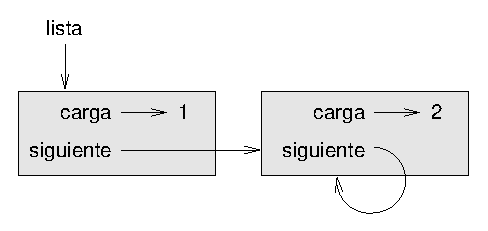
\includegraphics{illustrations/link4.eps}}
\afterfig

Si llamamos a  \texttt{imprimirLista} sobre esta lista, iteraría para
siempre. Si llamamos a \texttt{imprimirAlReves}, se haría recursión hasta
causar un error en tiempo de ejecución. Este comportamiento hace a las
listas circulares muy difíciles de manipular.

Sin embargo, a veces son muy útiles. Por ejemplo, podemos representar un 
número como una lista de dígitos y usar una lista infinita para representar
una fracción periódica.

Así que no es posible demostrar que  \texttt{imprimirLista} e
 \texttt{imprimirAlReves} terminen.  Lo mejor que podemos hacer es probar
la sentencia, ``Si la lista no tiene referencias hacia atrás, los métodos 
terminarán.''. Esto es una {\bf precondición}. Impone una restricción 
sobre los parámetros y describe el comportamiento del método si ésta
se cumple. Más adelante veremos otros ejemplos.

\index{precondición}


\section{El teorema de la ambigüedad fundamental}
\index{ambigüedad!teorema fundamental}
\index{teorema!fundamental de la ambigüedad}

Una parte de \texttt{imprimirAlReves} puede haber suscitado su curiosidad:


\beforeverb
\begin{verbatim}
    cabeza = lista
    resto = lista.siguiente
\end{verbatim}
\afterverb
%
Después de la primera asignación  \texttt{cabeza} y \texttt{lista} tienen 
el mismo tipo y el mismo valor. ¿Por qué creamos una nueva variable?

La respuesta yace en que las dos variables tienen roles distintos. 
\texttt{cabeza} es una referencia a un nodo y lista es una referencia 
a toda la lista. Estos ``roles'' están en la mente del programador y 
le ayudan a mantener la coherencia de los programas.

\index{variable!roles}
\index{rol!variable}

En general, no podemos decir inmediatamente qué rol juega una variable
en un programa. Esta ambigüedad puede ser útil, pero también dificulta
la lectura. Los nombres de las variables pueden usarse para documentar
la forma en que esperamos que se use una variable, y, a menudo, podemos
crear variables adicionates como \texttt{nodo} y \texttt{lista} para 
eliminar ambigüedades.

Podríamos haber escrito  \texttt{imprimirAlReves} de una manera más
concisa sin las variables \texttt{cabeza}  y \texttt{resto}, pero esto
también dificulta su lectura:

\beforeverb
\begin{verbatim}
def imprimirAlReves(lista) :
  if lista == None : 
     return
  imprimirAlReves(lista.siguiente)
  print lista,
\end{verbatim}
\afterverb
%
Cuando leamos el código, tenemos que recordar que {\tt imprimirAlReves} 
trata a su argumento como una colección y  \texttt{print} como a un 
solo nodo.

El  {\bf teorema de la ambigüedad fundamental} describe la ambigüedad
inherente en la referencia a un nodo:

\begin{quote}
{\bf Una variable que se refiera a un nodo puede tratar el nodo como 
un objeto único o como el acceso a la lista de nodos}
\end{quote}



\section{Modificando listas}
\index{lista!modificando}
\index{modificando listas}

Hay varias formas de modificar una lista enlazada. La obvia consiste en 
cambiar la carga de uno de sus nodos. Las mas interesantes son las que
agregan, eliminan o reordenan los nodos.

Como ejemplo, escribamos un método que elimine el segundo nodo en la 
lista y retorne una referencia al nodo eliminado

\beforeverb
\begin{verbatim}
def eliminarSegundo(lista):
  if lista == None: 
     return
  primero = lista
  segundo = lista.siguiente
  # hacemos que el primer nodo se refiera al tercero
  primero.siguiente = segundo.siguiente
  # desconectamos el segundo nodo de la lista
  segundo.siguiente = None
  return segundo
\end{verbatim}
\afterverb
%
Aquí también estamos usando variables temporales para aumentar la 
legibilidad. Aquí hay un ejemplo de uso del método:

\beforeverb
\begin{verbatim}
>>> imprimirLista(nodo1)
1 2 3
>>> borrado = eliminarSegundo(nodo1)
>>> imprimirLista(borrado)
2
>>> imprimirLista(nodo1)
1 3
\end{verbatim}
\afterverb
%
Este diagrama de estado muestra el efecto de la operación:

\beforefig
\centerline{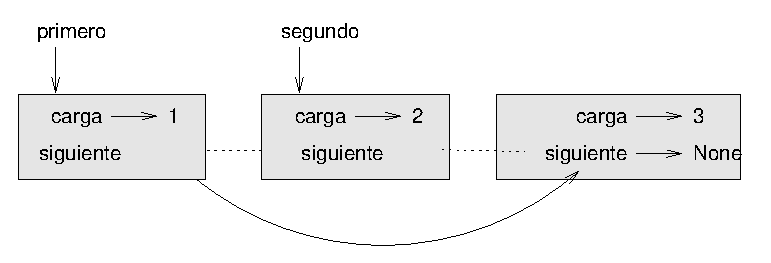
\includegraphics{illustrations/link5.eps}}
\afterfig

¿Qué pasa si usted llama este método con una lista que contiene un solo
elemento (un {\bf singleton})?  ¿Qué pasa si se llama con la lista vacía 
como argumento? ¿Hay precondiciones para este método? Si las hay, corríjalo
de forma que maneje de manera razonable las violaciones a la precondición.

\index{singleton}


\section{Funciones facilitadoras (wrappers) y auxiliares (helpers)}
\index{método facilitador}
\index{método!facilitador}
\index{función facilitadora}
\index{función!facilitadora}
\index{método auxiliar}
\index{método!auxiliar}

Es bastante útil dividir las operaciones de listas en dos métodos.
Con la impresión al revés podemos ilustrarlo, para desplegar  \texttt{[3, 2, 1]} 
en pantalla podemos llamar el método \texttt{imprimirAlReves} que 
desplegará \texttt{3, 2}, y llamar otro método para imprimir los
corchetes y el primer nodo. Nombrémosla así:

\beforeverb
\begin{verbatim}
def imprimirAlRevesBien(lista):
  print "[",
  if lista != None:
    cabeza = lista
    resto = lista.siguiente
    imprimirAlReves(resto)
    print cabeza,
  print "]",
\end{verbatim}
\afterverb
%
Es conveniente chequear que estos métodos funcionen bien para casos
especiales como la lista vacía o una lista con un solo elemento (singleton).

\index{singleton}

Cuando usamos este método en algún programa, llamamos directamente a la función
 \texttt{imprimirAlRevesBien}  para que llame a \texttt{imprimirAlReves}.  
En este sentido, \texttt{imprimirAlRevesBien} es una función {\bf facilitadora}, 
que utiliza a la otra, \texttt{imprimirAlReves} como función {\bf auxiliar}.


\section {La clase \texttt{ListaEnlazada}}
\index{ListaEnlazada}
\index{clase!ListaEnlazada}

Hay problemas más sutiles en nuestra implementación de listas que vamos 
a ilustrar desde los efectos a las causas, a partir de una implementación
alternativa exploraremos los problemas que resuelve.

Primero, crearemos una clase nueva llamada \texttt{ListaEnlazada}. Tiene
como atributos un entero con el número de elementos de la lista y una 
referencia al primer nodo. Las instancias de  \texttt{ListaEnlazada} sirven
como mecanismo de control de listas compuestas por instancias de la clase
 \texttt{Nodo}:

\beforeverb
\begin{verbatim}
class ListaEnlazada :
  def __init__(self) :
    self.numElementos = 0
    self.cabeza   = None
\end{verbatim}
\afterverb
%
Lo bueno de la clase \texttt{ListaEnlazada} es que proporciona un lugar
natural para definir las funciones facilitadores como 
\texttt{imprimirAlRevesBien} como métodos:

\beforeverb
\begin{verbatim}
class ListaEnlazada:
  ...
  def imprimirAlReves(self):
    print "[",
    if self.cabeza != None:
      self.cabeza.imprimirAlReves()
    print "]",

class Nodo:
  ...
  def imprimirAlReves(self):
    if self.siguiente != None:
      resto = self.siguiente
      resto.imprimirAlReves()
    print self.carga,
\end{verbatim}
\afterverb
%
Aunque inicialmente pueda parecer un poco confuso, vamos a renombrar a la función
 \texttt{imprimirAlRevesBien}.
Ahora vamos a implementar dos métodos con el mismo nombre \texttt{imprimirAlReves}: uno en la clase {\tt
Nodo}  (el auxiliar); y uno en la clase \texttt{ListaEnlazada} (el facilitador).
Cuando el facilitador llama al otro método, \texttt{self.cabeza.imprimirAlReves},
está invocando al auxiliar, porque \texttt{self.cabeza} es una instancia de
la clase \texttt{Nodo}.

Otro beneficio de la clase \texttt{ListaEnlazada} es que facilita agregar o eliminar
el primer elemento de una lista. Por ejemplo, \texttt{agregarAlPrincipio} es un método
de la clase \texttt{ListaEnlazada} que toma una carga como argumento y la pone
en un nuevo nodo al principio de la lista:

\beforeverb
\begin{verbatim}
class ListaEnlazada:
  ...
  def agregarAlPrincipio(self, carga):
    nodo = Nodo(carga)
    nodo.siguiente = self.cabeza
    self.cabeza = nodo
    self.numElementos = self.numElementos + 1
\end{verbatim}
\afterverb
%
Como de costumbre, usted debe revisar este código para verificar qué sucede con
los casos especiales. Por ejemplo, ¿qué pasa si se llama cuando la lista está vacía?


\section {Invariantes}
\index{Invariante}
\index{Invariante de objetos}
\index{lista!bien formada}

Algunas listas están ``bien formadas".  Por ejemplo, si una lista contiene un 
ciclo, causará problemas graves a nuestros métodos, así que deseamos 
evitar a toda costa que las listas tengan ciclos. Otro requerimiento de las listas
es que el número almacenado en el atributo \texttt{numElementos} de la clase
 \texttt{ListaEnlazada} sea igual al número de elementos en la lista.

Estos requerimientos se denominan  {\bf Invariantes} porque, idealmente, 
deberían ser ciertos para todo objeto de la clase en todo momento. Es una muy 
buena práctica especificar los Invariantes para los objetos porque permite
comprobar de manera mas sencilla la corrección del código, revisar la 
integridad de las estructuras de datos y detectar errores.

Algo que puede confundir acerca de los invariantes es que hay ciertos momentos
en que son violados. Por ejemplo, en el medio de  \texttt{agregarAlPrincipio}, 
después de que hemos agregado el nodo, pero antes de incrementar el atributo
 \texttt{numElementos}, el Invariante se viola. Esta clase de violación
es aceptable, de hecho, casi siempre es imposible modificar un objeto 
sin violar un Invariante, al menos momentáneamente. Normalmente, requerimos
que cada método que viole un invariante, lo establezca nuevamente.

Si hay una parte significativa de código en la que el Invariante se viola,
es importante documentarlo claramente, de forma que no se ejecuten operaciones
que dependan del Invariante.

\index{documentar}


\section{Glosario}
\index{referencia incrustada}
\index{referencia!incrustada}
\index{estructura de datos recursiva}
\index{estructura de datos!recursiva}
\index{lista enlazada}
\index{lista!enlazada}
\index{nodo}
\index{dato}
\index{enlace}
\index{precondición}
\index{invariante}
\index{facilitador}
\index{método auxiliar}
\index{teorema fundamental de la ambigüedad}
\index{singleton}

\begin{description}

\item[Referencia incrustada:] referencia almacenada en un
 atributo de un objeto.

\item[Lista enlazada:] es la estructura de datos que implementa
una  colección por medio de una secuencia de nodos enlazados.

\item[Nodo:] elemento de la lista, usualmente implementado
como un objeto que contiene una referencia hacia otro objeto
del mismo tipo.

\item[Carga:] dato contenido en un nodo.

\item[Enlace:] referencia incrustada, usada para enlazar un objeto con otro.

\item[Precondición:] condición lógica (o aserción) que debe ser
cierta para que un método funcione correctamente.

\item[Teorema fundamental de la ambigüedad:] la referencia a un nodo de
una lista puede interpretarse hacia un nodo determinado o como la referencia
a toda la lista de nodos.

\item[Singleton:] lista enlazada con un solo nodo.

\item[Facilitador:]  método que actúa como intermediario entre alguien
que llama un método y un método auxiliar. Se crean normalmente para
facilitar los llamados y hacerlos menos propensos a errores.

\item[Método auxiliar:] es un método que el programador no llama directamente, 
sino que es usado por otro método para  realizar parte
de una operación.

\item[Invariante:] aserción que debe ser cierta para un objeto
en todo momento (excepto cuando el objeto está siendo modificado).

\end{description}

